\documentclass[12pt]{article}

\usepackage[a4paper,left=25mm,right=25mm,top=35mm,bottom=25mm]{geometry}
\usepackage{ngerman}
\usepackage{parskip}
\usepackage{times}
\usepackage{graphicx}
\usepackage{listings}
\usepackage{fancyhdr}
\usepackage{float}
\usepackage{amsmath}

\setlength{\headheight}{15.2pt}
\pagestyle{fancy}

\lhead{Bildverarbeitung und Mustererkennung\\Praktikum Blatt 10}
\rhead{Patrick Hüntelmann\\24.06.2022}

\lstset{
  basicstyle=\ttfamily,
  breakatwhitespace=false,         % sets if automatic breaks should only happen at whitespace
  breaklines=true,                 % sets automatic line breaking
  captionpos=b,                    % sets the caption-position to bottom
  deletekeywords={...},            % if you want to delete keywords from the given language
  escapeinside={\%*}{*)},          % if you want to add LaTeX within your code
  extendedchars=true,              % lets you use non-ASCII characters; for 8-bits encodings only, does not work with UTF-8
  frame=single,	                   % adds a frame around the code
  keepspaces=true,                 % keeps spaces in text, useful for keeping indentation of code (possibly needs columns=flexible)
  language=python,                 % the language of the code
  showstringspaces=false,          % underline spaces within strings only
  showtabs=false,                  % show tabs within strings adding particular underscores
  tabsize=2,	                   % sets default tabsize to 2 spaces
}

\begin{document}

\pagenumbering{arabic}

\section*{Aufgabe 10}
Das k-means Clustering ist in der Funktion \textbf{kmeans} (main.py Zeile 11) implementiert. In dieser Funktion wird zunächst k-zufällige Clusterwerte erstellt. Anschließend wird in 10 Iterationen (festgelegt durch \textbf{MAX\_ITER}, Zeile 6) abwechselend der E-Schritt (Zeile 27-30) und der M-Schritt (Zeile 33-40) durchgeführt. Zum Schluß werden die Cluster auf ein Ergebnisbild übertragen.

In der Funktion \textbf{main} wird das Clustering aufgerufen. Hier wird Bild geladen und für $k = 2$ und $k = 4$ das Clustering auf einem Farbbild und einem Grauwertbild durchgeführt und das Ergebnis dargestellt.

\subsubsection*{Ergebnisbilder}
\begin{figure}[H]
  \centering
  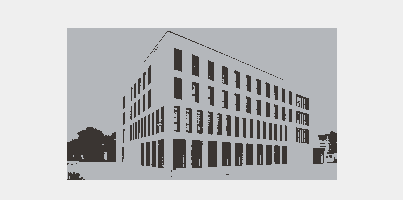
\includegraphics[width=0.7\textwidth, keepaspectratio]{color2.png}\\
  Farbbild, $k = 2$
\end{figure}
\begin{figure}[H]
  \centering
  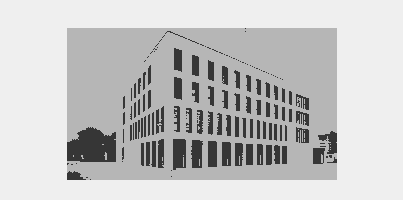
\includegraphics[width=0.7\textwidth, keepaspectratio]{gray2.png}\\
  Grauwertbild, $k = 2$
\end{figure}
\begin{figure}[H]
  \centering
  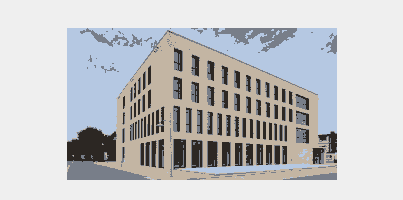
\includegraphics[width=0.7\textwidth, keepaspectratio]{color4.png}\\
  Farbbild, $k = 4$
\end{figure}
\begin{figure}[H]
  \centering
  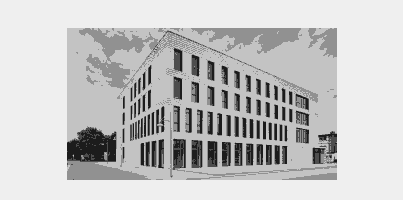
\includegraphics[width=0.7\textwidth, keepaspectratio]{gray4.png}\\
  Grauwertbild, $k = 4$
\end{figure}

\end{document}
